\section{DRTA sonda}
    \subsection{Princip fungování} \label{sec:DRTA-princip}
        Myšlenka stojící za DRTA sondou se opírá právě o měření rovnovážných teplot (viz předchozí Kapitola \ref{sec:mereni-teplot}). Budeme-li uvažovat teplotní čidlo s restitučním faktorem $f_A$, pak bude měřená teplota $T_{rA}$ dána následovně:
        \begin{equation} \label{eq:trA}
            T_{rA} = T + f_A \frac{u^2}{2 c_p}
        \end{equation}
        \noindent Jednoduchou úpravou lze odvodit vztah pro určení rychlosti proudění:
        \begin{equation} \label{eq:rychlost-jenom-A}
            u = \sqrt{2 c_p \frac{T_{rA} - T}{f_A}}
        \end{equation}
        Takový postup by však vyžadoval znalost statické teploty nabíhajícího proudu $T$, nebo potažmo teploty klidové $T_0$ – tuto metodiku lze najít v řadě aplikací (viz metoda RTA – \textit{Recovery Temperature Anemometry} \cite{Ishibashi2004, Ishibashi2012}). Zde byl k měření použit termočlánek s restitučním faktorem uvažovaným jako $\sqrt{Pr}$ a výsledná rychlost proudění byla stanovena ze vztahu:
        \begin{equation}
            u = \sqrt{\frac{2 \kappa r}{\kappa - 1} \frac{T_0 - T_{rA}}{f_A}}
        \end{equation}
        
        Nevýhodou výše uvedené RTA metody je právě nutnost měření dalších parametrů proudění ($T$, $T_0$), což značně omezuje možnosti jejího využití. Klíčovým krokem v návrhu DRTA sondy je proto eliminace statické teploty ze Vztahu \ref{eq:rychlost-jenom-A}. Toho lze docílit použitím odlišného teplotního čidla – odlišnost je zde reprezentovaná rozdílným restitučním faktorem, který označme $f_B$. Toto čidlo bude tedy indikovat teplotu $T_{rB}$:
        \begin{equation} \label{eq:trB}
            T_{rB} = T + f_B \frac{u^2}{2 c_p}
        \end{equation}
        \noindent Rychlost proudění lze následně určit z rozdílu Vztahů \ref{eq:trA} a \ref{eq:trB}:
        \begin{equation} \label{eq:mereni-rychlosti}
            \begin{split} 
                T_{rA} - T_{rB} = \brac{f_A - f_b} \frac{u^2}{2 c_p} \\
                u = \sqrt{\frac{2 c_p \brac{T_{rA} - T_{rB}}}{\brac{f_A - f_b}}}
            \end{split}
        \end{equation}

        Výhoda použití dvou teplotních snímačů s rozdílnými restitučními faktory spočívá navíc v tom, že lze obdobně odvodit i vztahy pro určení Machova čísla a statické teploty nabíhajícího proudu. Pro určení $\Ma$ je třeba nejprve upravit Vztahy \ref{eq:trA} a \ref{eq:trB}:
        \begin{align}
            \begin{split}
                T_{rA} &= T + f_A \frac{u^2}{2 c_p} \frac{a^2}{a^2} = T \brac{1 + f_A \frac{\kappa - 1}{2} \Ma ^2} \\
                T_{rB} &=  T \brac{1 + f_B \frac{\kappa - 1}{2} \Ma ^2}
            \end{split}
        \end{align}
        \noindent Výsledný vztah pro $\Ma$ vznikne z podílu měřených teplot:
        \begin{align}
            \begin{split}
                \frac{T_{rA}}{T_{rB}} &= \frac{1 + f_A \frac{\kappa - 1}{2} \Ma ^2}{1 + f_B \frac{\kappa - 1}{2} \Ma ^2} \\
                \Ma &= \sqrt{\frac{2}{\kappa - 1} \frac{T_{rA}-T_{rB}}{T_{rB} f_A - T_{rA} f_B}}
            \end{split}
        \end{align}
        \noindent Určení statické teploty lze odvodit pomocí eliminace rychosti proudění ze Vztahů \ref{eq:trA} a \ref{eq:trB}:
        \begin{align}
            \begin{split}
                \frac{u^2}{2 c_p} &= \frac{T_{rA} - T}{f_A} = \frac{T_{rB} - T}{f_B} \\
                T &= \frac{T_{rB} f_A - T_{rA} f_B}{f_A - f_B}
            \end{split}
        \end{align}

        

        \vspace{10cm}

        Princip měření rychlosti pomocí DRTA sondy (DRTA = \uv{\textit{Double Recovery Temperature Anemometry}}) spočívá ve využití dvou teplotních čidel, v tomto návrhu bylo pracováno s odporovými teplotními snímači Pt100. Komplikaci při použití jediného snímače pro určení rychlosti proudění představuje nutná znalost statické teploty. Ta lze jednoduše eliminovat přidáním druhého snímače s rozdílným restitučním faktorem:
        \begin{align}
            T_{rA} &= T + f_A \frac{u^2}{2 c_p} \\
            T_{rB} &= T + f_B \frac{u^2}{2 c_p} \\
            T_{rA} - T_{rB} &= \brac{f_A - f_b} \frac{u^2}{2 c_p} \\
            u &= \sqrt{\frac{2 c_p \brac{T_{rA} - T_{rB}}}{\brac{f_A - f_b}}} \label{eq:mereni-rychlosti}             
        \end{align}
        \noindent kde indexy $A$, respektive $B$ odpovídají jednotlivým čidlům. Podobným způsobem lze sestavit vztah pro určení Machova čísla:
        \begin{align}
            T_{rA} &= T + f_A \frac{u^2}{2 c_p} \frac{a^2}{a^2} = T \brac{1 + f_A \frac{\kappa - 1}{2} \Ma ^2} \\
            T_{rB} &=  T \brac{1 + f_B \frac{\kappa - 1}{2} \Ma ^2} \\
            \frac{T_{rA}}{T_{rB}} &= \frac{1 + f_A \frac{\kappa - 1}{2} \Ma ^2}{1 + f_B \frac{\kappa - 1}{2} \Ma ^2} \\
            \Ma &= \sqrt{\frac{2}{\kappa - 1} \frac{T_{rA}-T_{rB}}{T_{rB} f_A - T_{rA} f_B}}
        \end{align}

    \subsection{Výchozí geometrie}
        Zkoumaná sonda se skládá z dvou odporových teplotní čidel Pt100 (model \textit{1PT100K2515}) o průměru $1.5 \unit{mm}$ a délce $25 \unit{mm}$. Ty jsou umístěny rovnoběžně ve směru proudění pomocí těsnění na jejich koncích, ukotveného v mosazné trubici o průměru $4 \Unit{mm}$ a tloušťce $0.4 \Unit{mm}$, která je využita zároveň k dosažení rozdílu restitučních faktorů jednotlivých čidel. Prostorové uspořádání sestavy je patrné z obrázku \ref{fig:vychozi-DRTA}. Vyšším restitučním faktorem disponuje čidlo umístěné uvnitř trubice a dále v práci o něm bude hovořeno jako o čidlu A. Proudění stíněním čidla A umožňují dva odvětrávací otvory umístěné $12 \Unit{mm}$ od vstupu do trubice. Čidlo umístěné volně v proudícím médiu vykazuje nižší restituční faktor a bude dále značeno jako čidlo B.
        
        \begin{figure}[ht!]
            \centering
            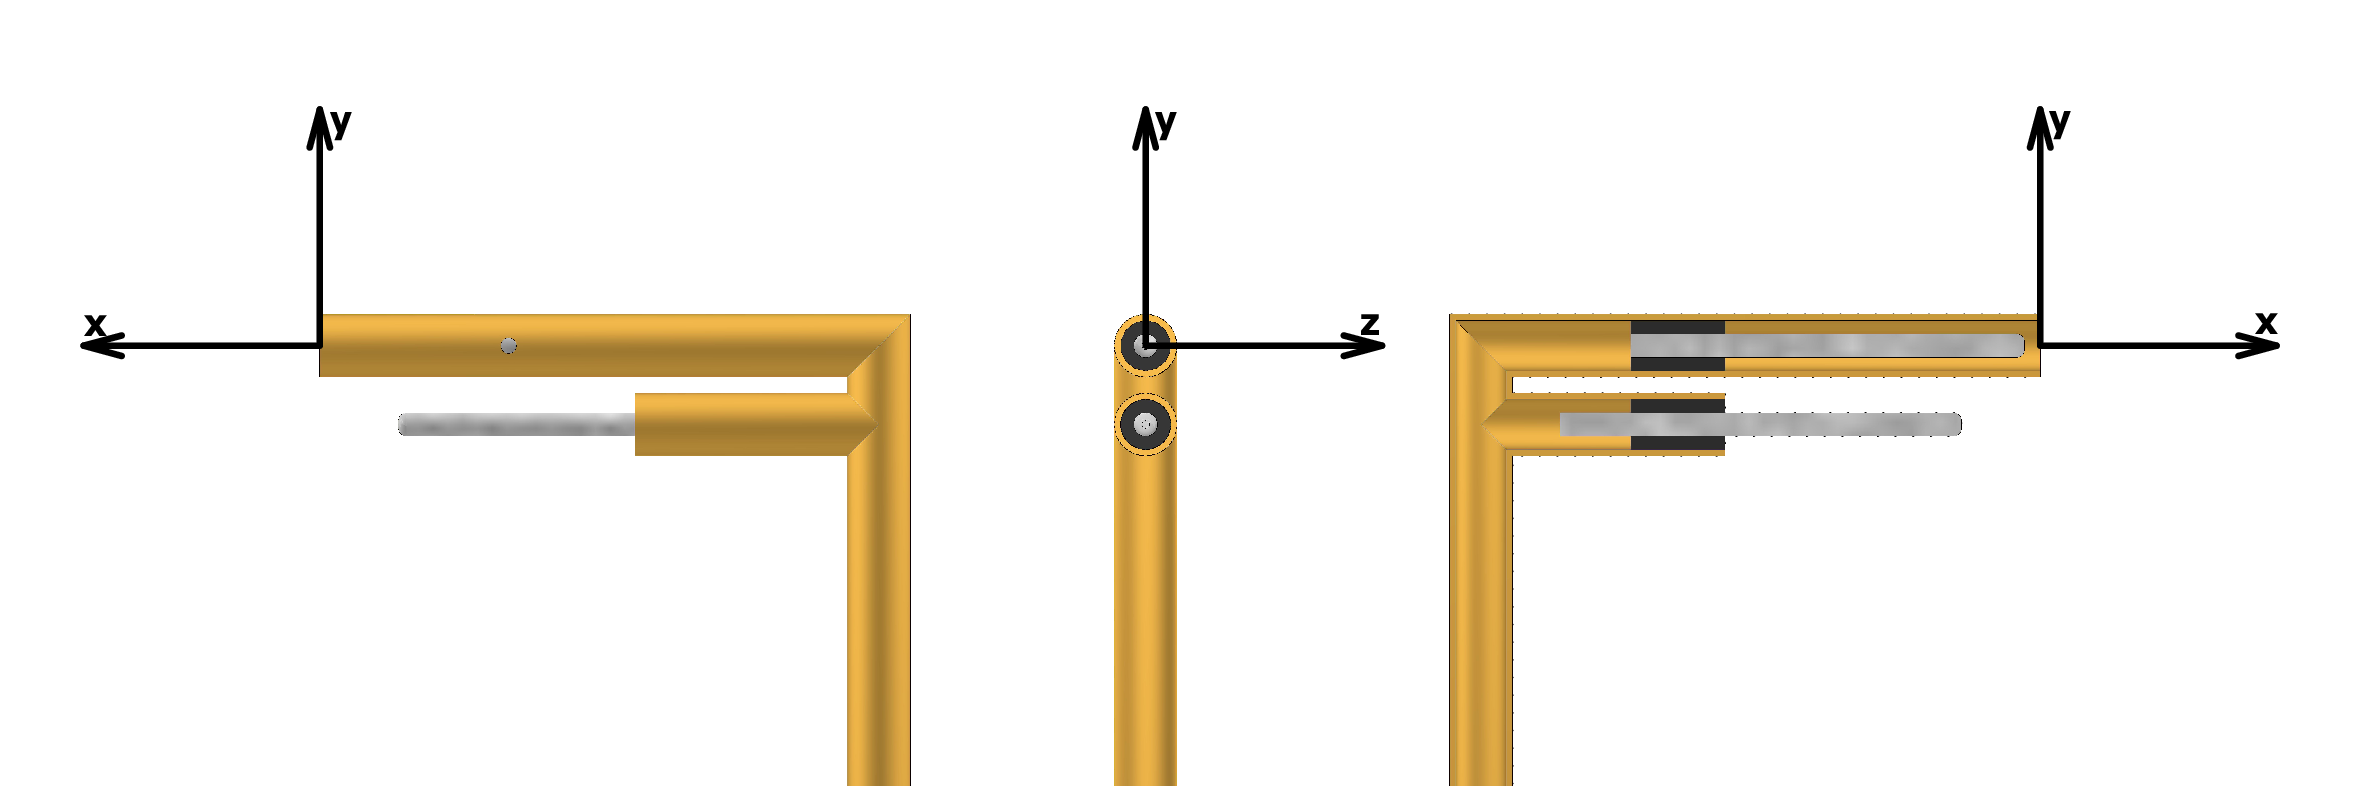
\includegraphics[width=\textwidth]{200_DRTA_SONDA/Vychozi_DRTA.png}
            \caption{Výchozí geometrie DRTA sondy.}
            \label{fig:vychozi-DRTA}
        \end{figure}
    \subsection{Cíle numerických simulací}
        